\documentclass{beamer}

% chktex-file 1
% chktex-file 8

\usetheme[workplace=fi]{MU}
\usepackage[utf8]{inputenc}
\usepackage[
  main=czech,
  english
]{babel}
\usepackage[utf8]{inputenc}
\usepackage[T1]{fontenc}
\usepackage{csquotes}
\usepackage{booktabs}
\usepackage{amsmath}

\newcommand{\RR}{\ensuremath{\mathbb{R}}}

\usepackage{tikz}
\usetikzlibrary{arrows, shapes.geometric}

\newlength{\nodesize}
\setlength{\nodesize}{1.5em}
\tikzset{and/.style = {shape=circle,draw,minimum size=\nodesize}}
\tikzset{or/.style = {shape=rectangle,draw,minimum size=\nodesize}}

\tikzset{min/.style = {shape=circle,draw,minimum size=\nodesize}}
\tikzset{max/.style = {shape=rectangle,draw,minimum size=\nodesize}}
\tikzset{rand/.style = {diamond,draw,minimum size=\nodesize}}

\tikzset{edge/.style = {->,> = latex'}}

% Allows for split by delimiter
% \getNth{string}{delimiter}{entry_no}
% Source: https://tex.stackexchange.com/questions/12810/how-do-i-split-a-string
\ExplSyntaxOn
\NewDocumentCommand{\getNth}{mmm}
  {
    % #1 string, #2 separator, #3 index
    \seq_set_split:Nnx \l_tmpa_seq { #2 } { #1 }
    \seq_item:Nn \l_tmpa_seq { #3 }
  }
\ExplSyntaxOff

\setbeamertemplate{enumerate item}{\alph{enumi})}  % chktex 9 chktex 10

\newcommand{\tictactoe}[2]{%
    \draw (#1.center) ++(-.5,-.5) -- +(0,1);
    \draw (#1.center) ++(-.1667,-.5) -- +(0,1);
    \draw (#1.center) ++(.1667,-.5) -- +(0,1);
    \draw (#1.center) ++(.5,-.5) -- +(0,1);
    \draw (#1.center) ++(-.5,-.5) -- +(1,0);
    \draw (#1.center) ++(-.5,-.1667) -- +(1,0);
    \draw (#1.center) ++(-.5,.1667) -- +(1,0);
    \draw (#1.center) ++(-.5,.5) -- +(1,0);
    \draw (#1.center) ++(-.3333,.3333) node {\getNth{#2}{;}{1}};
    \draw (#1.center) ++(0,.3333) node {\getNth{#2}{;}{2}};
    \draw (#1.center) ++(.3333,.3333) node {\getNth{#2}{;}{3}};
    \draw (#1.center) ++(-.3333,0) node {\getNth{#2}{;}{4}};
    \draw (#1.center) ++(0,0) node {\getNth{#2}{;}{5}};
    \draw (#1.center) ++(.3333,0) node {\getNth{#2}{;}{6}};
    \draw (#1.center) ++(-.3333,-.3333) node {\getNth{#2}{;}{7}};
    \draw (#1.center) ++(0,-.3333) node {\getNth{#2}{;}{8}};
    \draw (#1.center) ++(.3333,-.3333) node {\getNth{#2}{;}{9}};
}

\title{Hry a herní strategie}
\author{Jindřich Matuška}
\institute[FI MU]{Faculty of Informatics, Masaryk University}
\date{24. října 2024}

\AtBeginSection[]
{
    \begin{frame}
        \frametitle{Obsah}
        \tableofcontents[currentsection]
    \end{frame}
}

\begin{document}

\frame{\titlepage}

\frame{
    \frametitle{Čas na odpovědníky}
}

\begin{frame}
    \frametitle{Obsah}
    \tableofcontents
\end{frame}

\begin{section}{MINIMAX graf, algoritmus}

\frame{
    \frametitle{MINIMAX graf}
    Syntax
    \begin{itemize}
        \item orientovaný graf
        \item vnitřní vrcholy typu \textbf{MIN} nebo \textbf{MAX}
            \begin{itemize}
                \item značíme kolečkem (MIN) či čtverečkem (MAX)
            \end{itemize}
        \item koncové vrcholy s přiřazenou hodnotou z $\mathbb{R}\cup \{-\infty, \infty\}$
    \end{itemize}
}

\frame{
    \frametitle{MINIMAX algoritmus}
    \begin{itemize}
        \item Rekurzivní algoritmus
        \item Hodnota listů daná definicí stromu
        \item Hodnota vrcholu MIN je nejmenší hodnota z následníků
        \item Hodnota vrcholu MAX je největší hodnota z následníků
            \vspace{1em}
        \item Odpovídá hře s nulovým součtem 2 hráčů
        \item Hráči se střídají
    \end{itemize}
    \begin{equation*}
        minimax(X) = \left\{
            \begin{matrix}
                \max_{n\in X^\rightarrow} minimax(n) & \text{ pokud }X\text{ je MAX uzel}\\
                \min_{n\in X^\rightarrow} minimax(n) & \text{ pokud }X\text{ je MIN uzel}
            \end{matrix}
            \right.
    \end{equation*}
}

\frame{
    \frametitle{Příklad}
\begin{center}
    \begin{tikzpicture}
        \node[min] (a) at (0,0) {};
        \node[max] (b) at (-2,-1) {};
        \draw[edge] (a) to (b);
        \node[max] (c) at (2,-1) {};
        \draw[edge] (a) to (c);
        \node[min] (d) at (-3,-2) {};
        \draw[edge] (b) to (d);
        \node[min] (e) at (-1,-2) {};
        \draw[edge] (b) to (e);
        \node[min] (f) at (1,-2) {};
        \draw[edge] (c) to (f);
        \node[min] (g) at (3,-2) {};
        \draw[edge] (c) to (g);
        \node[max] (h) at (-3.5,-3) {$7$};
        \draw[edge] (d) to (h);
        \node[max] (i) at (-2.5,-3) {$-5$};
        \draw[edge] (d) to (i);
        \node[max] (h) at (-1.5,-3) {$-\infty$};
        \draw[edge] (e) to (h);
        \node[max] (i) at (-.5,-3) {$0$};
        \draw[edge] (e) to (i);
        \node[max] (h) at (1,-3) {$5$};
        \draw[edge] (f) to (h);
        \node[max] (i) at (3,-3) {$\infty$};
        \draw[edge] (g) to (i);
    \end{tikzpicture}
\end{center}
}

\frame{
    \frametitle{MINIMAX pro popis her}
    \hfill
    \begin{tikzpicture}[scale=2]
        \node (a) at (-2,0) {};
        \tictactoe{a}{;x;;o;x;o;;x;o}
        \node at (-2,-1) {-1};
        \node (a) at (0,0) {};
        \tictactoe{a}{x;o;x;o;x;o;o;x;o}
        \node at (0,-1) {0};
        \node (a) at (2,0) {};
        \tictactoe{a}{x;x;o;o;o;o;x;x;o}
        \node at (2,-1) {1};
    \end{tikzpicture}
    \hfill\phantom{}
}

\frame{
    \frametitle{Příklad 4.1.1}
    Rozhodněte, zda je následující hry možné modelovat MINIMAX stromy.
    Pokud ano, zamyslete se nad tím, jak by takové stromy vypadaly.
    \begin{enumerate}
        \item šachy
        \item sudoku
        \item piškvorky na neomezené hrací ploše
        \item kámen, nůžky, papír
        \item tenis
    \end{enumerate}
}  % chktex 10

\frame{
    \frametitle{Příklad 4.1.2}
    Doplňte nějaké konkrétní ohodnocení koncových stavů her s naznačeným
    MINIMAX stromem tak, aby začínající hráč dosáhl nejlepšího možného výsledku hraním
    zadaných strategií, předpokládáme-li, že jeho soupeř nedělá chyby.
    Jaké vztahy obecně musí v takovém případě platit pro hodnoty listů?

    \begin{enumerate}[<only@+>]  % chktex 9
        \item Výherní strategie nechť je \textit{left}
            \begin{center}
            \begin{tikzpicture}
                \node[max] (a) at (0,0) {};
                \node[min] (b) at (-2,-1) {};
                \draw[edge] (a) -- (b) node [midway, above] {left};
                \node[min] (c) at (2,-1) {};
                \draw[edge] (a) -- (c) node [midway, above] {right};
                \node[max] (d) at (-3,-2) {$a$};
                \draw[edge] (b) to (d);
                \node[max] (e) at (-1,-2) {$b$};
                \draw[edge] (b) to (e);
                \node[max] (f) at (1,-2) {$c$};
                \draw[edge] (c) to (f);
                \node[max] (g) at (3,-2) {$d$};
                \draw[edge] (c) to (g);
            \end{tikzpicture}
            \end{center}
        \item Výherní strategie nechť je volit \textit{left} v prvním kole
            a \textit{blue} ve druhém. Nezapomeňte zařídit, aby nás dokonalý soupeř
            s jistotou dovedl k volbě potřebné strategie.
            \begin{center}
            \begin{tikzpicture}
                \node[max] (a) at (0,0) {};
                \node[min] (b) at (-2,-1) {};
                \draw[edge] (a) -- (b) node [midway, above] {left};
                \node[min] (c) at (2,-1) {};
                \draw[edge] (a) -- (c) node [midway, above] {right};
                \node[max] (d) at (-3,-2) {};
                \draw[edge] (b) -- (d);
                \node[max] (e) at (-1,-2) {};
                \draw[edge] (b) -- (e);
                \node[max] (f) at (2,-2) {};
                \draw[edge] (c) -- (f);
                \node[max] (h) at (-3,-3) {$a$};
                \draw[edge] (d) -- (h);
                \node[min] (i) at (-1.5,-3) {$b$};
                \draw[edge] (e) -- (i) node [midway, above left] {blue};
                \node[min] (j) at (-.5,-3) {$c$};
                \draw[edge] (e) -- (j) node [midway, above right] {red};
                \node[min] (k) at (1.5,-3) {$d$};
                \draw[edge] (f) -- (k);
                \node[min] (l) at (2.5,-3) {$e$};
                \draw[edge] (f) -- (l);
            \end{tikzpicture}
            \end{center}
    \end{enumerate}
}  % chktex 10

\frame{
    \frametitle{Příklad 4.1.3}
    Dokažte, že MINIMAX stromy rozšiřují AND/OR stromy. Jinými slovy
    ukažte, že každý AND/OR strom lze chápat jako MINIMAX strom.
}

\end{section}

\begin{section}{Jupyter lab}
\frame{
    \frametitle{Implementace MINIMAX algoritmu}
    Implementujte MINIMAX algoritmus na příkladu $3\times3$ piškvorek.
}
\end{section}

\begin{section}{Alfa-beta prořezávání}

\frame{
    \frametitle{Příklad}
    \begin{center}
    \begin{tikzpicture}
        \node[max] (a) at (0,0) {};
        \node[min] (b) at (-2,-1) {};
        \draw[edge] (a) -- (b);
        \node[min] (c) at (2,-1) {};
        \draw[edge] (a) -- (c);
        \node[max] (d) at (-3,-2) {$2$};
        \draw[edge] (b) to (d);
        \node[max] (e) at (-1,-2) {$3$};
        \draw[edge] (b) to (e);
        \node[max] (f) at (1,-2) {$4$};
        \draw[edge] (c) to (f);
        \node[max] (m) at (2,-2) {$1$};
        \draw[edge] (c) to (m);
        \node[max] (g) at (3,-2) {$2$};
        \draw[edge] (c) to (g);
    \end{tikzpicture}
    \end{center}
}

\frame{
    \frametitle{ALFA-BETA prořezávání}
    \begin{itemize}
        \item Nepotřebujeme prohledávat všechny uzly
        \item Pamatujeme si parametry $\alpha$ (alespoň), $\beta$ (nejvýše)
        \item V uzlu MAX aktualizujeme $\alpha$, v MIN $\beta$
        \item Parametry posováme v DFS prohledávání
    \end{itemize}
    \vfill
    \begin{center}
    \begin{tikzpicture}
        \node[max] (a) at (0,0) {};
        \node[min] (b) at (-2,-1) {};
        \draw[edge] (a) -- (b);
        \node[min] (c) at (2,-1) {};
        \draw[edge] (a) -- (c);
        \node[max] (d) at (-3,-2) {$2$};
        \draw[edge] (b) to (d);
        \node[max] (e) at (-1,-2) {$3$};
        \draw[edge] (b) to (e);
        \node[max] (f) at (1,-2) {$4$};
        \draw[edge] (c) to (f);
        \node[max] (m) at (2,-2) {$1$};
        \draw[edge] (c) to (m);
        \node[max] (g) at (3,-2) {$2$};
        \draw[edge] (c) to (g);
    \end{tikzpicture}
    \end{center}
}

\frame{
    \frametitle{Příklad 4.2.2}
    \only<1>{
    Zadaný strom MINIMAX střídá po úrovních typy svých uzlů a každý
    jeho list je ve stejné hloubce. Takové v literatuře (a hlavně v praxi)
    budete vídat nejčastěji, neboť přirozeně vznikají při modelování
    mnoha zajímavých her. Jako v celém zbytku sbírky
    předpokládejte i zde, že algoritmus prochází vrcholy v pořadí zleva doprava.}
    \only<2->{
        \begin{enumerate}[<only@+>]
            \item 
            \setcounter{enumi}{0}
            \item Vyřešte strom s pomocí algoritmu ALFA-BETA.\@
                Především tedy zjistěte výslednou
                hodnotu kořene a které podstromy budou uřezány,
                tj.\ nebudou vůbec navštíveny.
                Při výpočtu věnujte zvláštní pozornost tomu,
                abyste porozuměli, jakým způsobem $\alpha$
                odpovídá dolní hranici a $\beta$ naopak horní.
            \item Při zachování struktury grafu navrhněte vhodné
                hodnoty listů tak, aby nedošlo k žádnému prořezávání
                (a algoritmus tedy navštívil všechny listy).
            \item Při zachování struktury grafu navrhněte vhodné hodnoty listů
                tak, aby došlo k největšímu možnému prořezávání
                (a algoritmus tedy navštívil co nejméně uzlů).
        \end{enumerate}
    }
    \vfill
    \begin{center}
    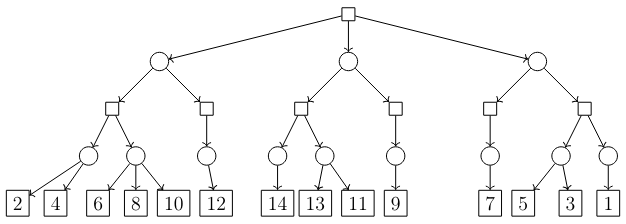
\includegraphics[width=.8\textwidth]{sources/graph_big.png}
    \end{center}
}

\frame{
    \frametitle{Příklad 4.2.3}
    Při kterých z následujících transformací MINIMAX stromu může dojít
    ke změně nalezené optimální strategie?
    \begin{enumerate}
        \item Ke všem hodnotám listů přičteme stejnou reálnou konstantu c.
        \item Všechny hodnoty v listech vynásobíme stejnou konstantou c.
        \item Hodnoty ve všech listech se libovolně změní tak,
            aby mezi nimi zůstalo zachováno jejich
            původní uspořádání.
        \item Všechny uzly typu MIN změníme na MAX a naopak.
            Hodnoty v listech pronásobíme -1.
    \end{enumerate}
}

\end{section}

\begin{section}{Neterministické hry}

\frame{
    \frametitle{Nedeterminismus}
    \begin{itemize}
        \item nový typ vrcholu RAND
            \begin{itemize}
                \item značíme kosočtvercem
                \item hrany z něj vycházející jsou ohodnoceny pravděpodobností
            \end{itemize}
        \item Hodnota RAND vrcholu je váženým součtem
    \end{itemize}
    \begin{equation*}
        minimax(X) = \left\{
            \begin{matrix}
                \max_{n\in X^\rightarrow} minimax(n) & \text{ pokud }X\text{ je MAX uzel}\\
                \min_{n\in X^\rightarrow} minimax(n) & \text{ pokud }X\text{ je MIN uzel}\\
                \sum_{n\in X^{\rightarrow}} minimax(n) \cdot P(n) & \text{ pokud }X\text{ je RAND uzel}
            \end{matrix}
            \right.
    \end{equation*}
}

\frame{
    \frametitle{Příklad}
    \begin{center}
        \begin{tikzpicture}
            \node[max] (a) at (0,0) {};
            \node[rand] (b) at (-3,-1) {};
            \draw[edge] (a) -- (b) node [midway, above left] {red};
            \node[min] (d) at (-4,-2) {};
            \draw[edge] (b) -- (d) node [midway, above left] {orel/0.5};
            \node[min] (e) at (-2,-2) {};
            \draw[edge] (b) -- (e) node [midway, above right] {panna/0.5};
            \node[max] (h) at (-4.5,-3) {$1$};
            \draw[edge] (d) -- (h) node [midway, above left] {blue};
            \node[max] (h) at (-3,-3) {$-1$};
            \draw[edge] (e) -- (h) node [midway, above left] {red};
            \node[max] (i) at (-1.5,-3) {$1$};
            \draw[edge] (e) -- (i) node [midway, above right] {blue};
            \node[rand] (b) at (3,-1) {};
            \draw[edge] (a) -- (b) node [midway, above right] {red};
            \node[min] (d) at (2,-2) {};
            \draw[edge] (b) -- (d) node [midway, above left] {orel/0.5};
            \node[min] (e) at (4,-2) {};
            \draw[edge] (b) -- (e) node [midway, above right] {panna/0.5};
            \node[max] (h) at (1.5,-3) {$-1$};
            \draw[edge] (d) -- (h) node [midway, above left] {blue};
            \node[max] (h) at (3,-3) {$1$};
            \draw[edge] (e) -- (h) node [midway, above left] {red};
            \node[max] (i) at (4.5,-3) {$-1$};
            \draw[edge] (e) -- (i) node [midway, above right] {blue};
        \end{tikzpicture}
    \end{center}
}

\end{section}

\begin{section}{Jupyter lab}
\frame{
    \frametitle{Implementace ALFA-BETA prořezávání}
    Implementujte ALFA-BETA prořezávání na příkladu $3\times3$ piškvorek.

    Můžete s výhodou využít již vytvořený MINIMAX algoritmus
}
\end{section}

\end{document}  % chktex 17
